\begin{figure}
	\tikzsetnextfilename{intorno-circolare-r2}
	\centering
	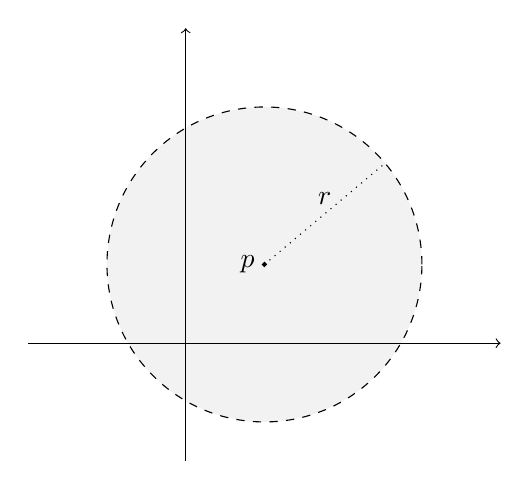
\begin{tikzpicture}
		\draw[dashed,fill=gray!10] (0,0) circle (2);
		\draw[->] (-3,-1) -- (3,-1);
		\draw[->] (-1,-2.5) -- (-1,3);
		\draw (0,0) node[left]{$p$};
		\draw[fill=black] (0,0) circle (.025);
		\draw[dotted] (0,0) to node[anchor=south]{$r$} (40:2);
	\end{tikzpicture}
	\caption{Un intorno $B(\vec p,r)\subset(\R^2,\norm{\cdot})$.}
	\label{fig:B-circ}
\end{figure}
